\chapter[Resultados Preliminares]{Resultados Preliminares}
\label{sec:Resultados}

\section{Resultados de Filtragem}

Nesta seção, são apresentados os resultados obtidos a partir de ensaios realizados em um ambiente virtual \textit{PureData}, simulando filtragem em diferentes frequências de corte.

Para a análise, foram utilizadas duas músicas: \cite{track01} e \cite{track02}. Selecionou-se uma janela de duração de dois segundos de cada música, considerando que esse intervalo capturava elementos de todas as bandas de frequência. Sobre essas janelas, foi aplicado um sistema de filtragem composto por filtros passa-altas.

As frequências de corte selecionadas foram:

\begin{itemize}
    \item 0 Hz
    \item 20 Hz
    \item 300 Hz
    \item 4 kHz
    \item 24 kHz
\end{itemize}

Para cada frequência de corte, foi analisado o comportamento do sinal tanto no domínio do tempo quanto no domínio da frequência, utilizando a Transformada de Fourier de Curto Termo (STFT - \textit{Short Time Fourier Transform}). Os pares de representações em função da frequência de corte, consolidadas na música, foram aplicados às duas músicas de referência.

\begin{figure}[h]
	\centering
    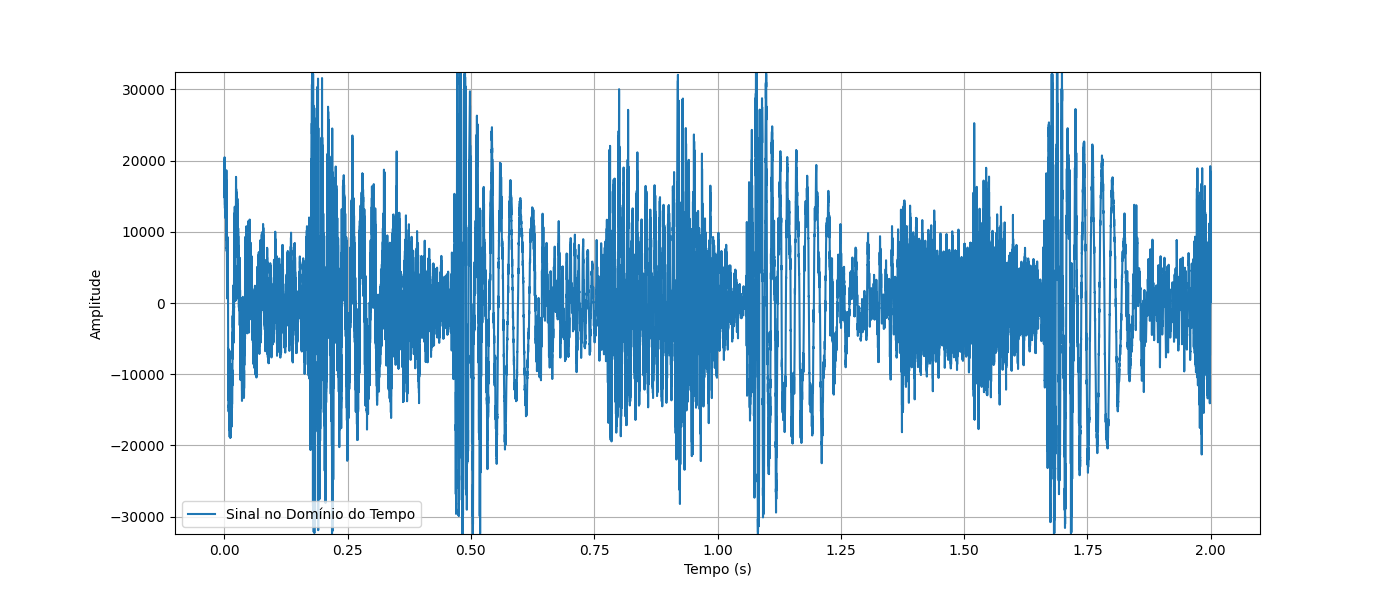
\includegraphics[width=0.5\textwidth]{figuras/fig40.png}
	\caption{música 1 no domínio do tempo sem filtragem}
	\label{fig40}
\end{figure}

Na Figura \ref{fig40}, vê-se a janela do arquivo de áudio no domínio do tempo, com a presença de \textit{kicks} e elementos de maiores frequências. A Figura \ref{fig41} mostra a STFT dessa janela, revelando maior presença de elementos em baixa frequência, assim como variações de elementos de agudos conforme a música avança.

\begin{figure}[h]
	\centering
    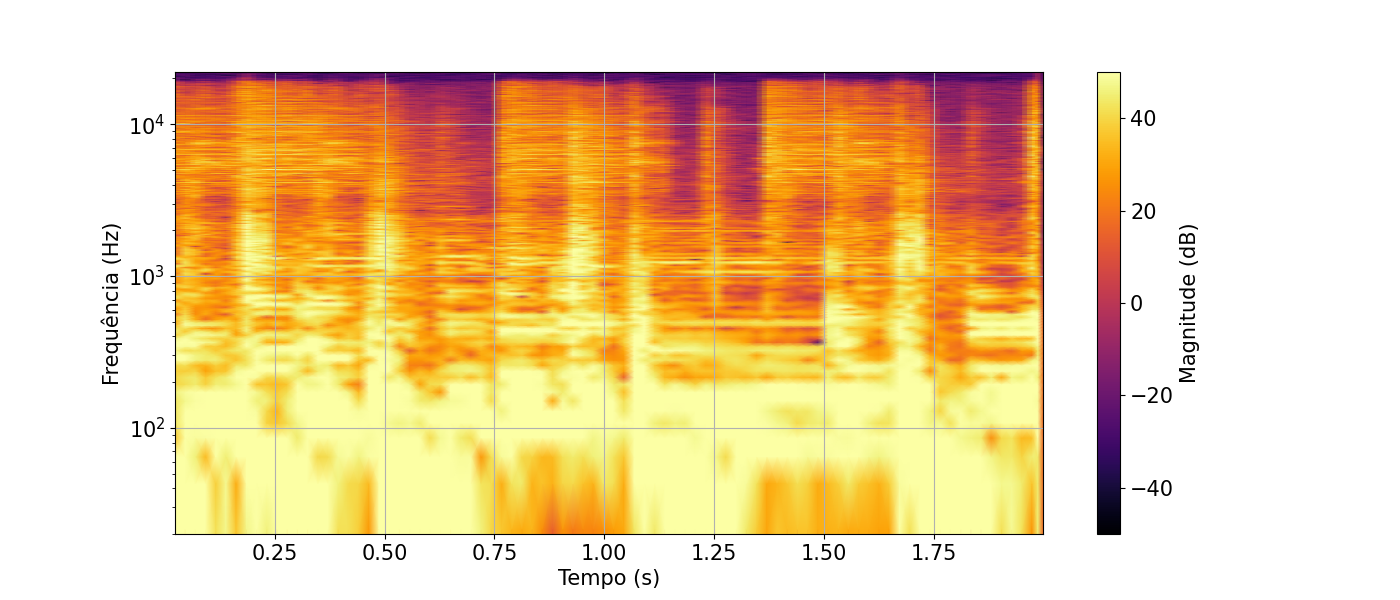
\includegraphics[width=0.5\textwidth]{figuras/fig41.png}
	\caption{música 1 no domínio da frequência sem filtragem}
	\label{fig41}
\end{figure}

As próximas figuras correspondem à aplicação de filtros passa-altas.

Um filtro passa-altas de 20 Hz foi aplicado ao sinal, como mostrado na Figura \ref{fig24}, onde as alterações no sinal são sutis. A Figura \ref{fig25} confirma que não houve grandes alterações nas componentes de frequência após a aplicação do filtro com frequência de corte de 20 Hz.

\begin{figure}[h]
	\centering
    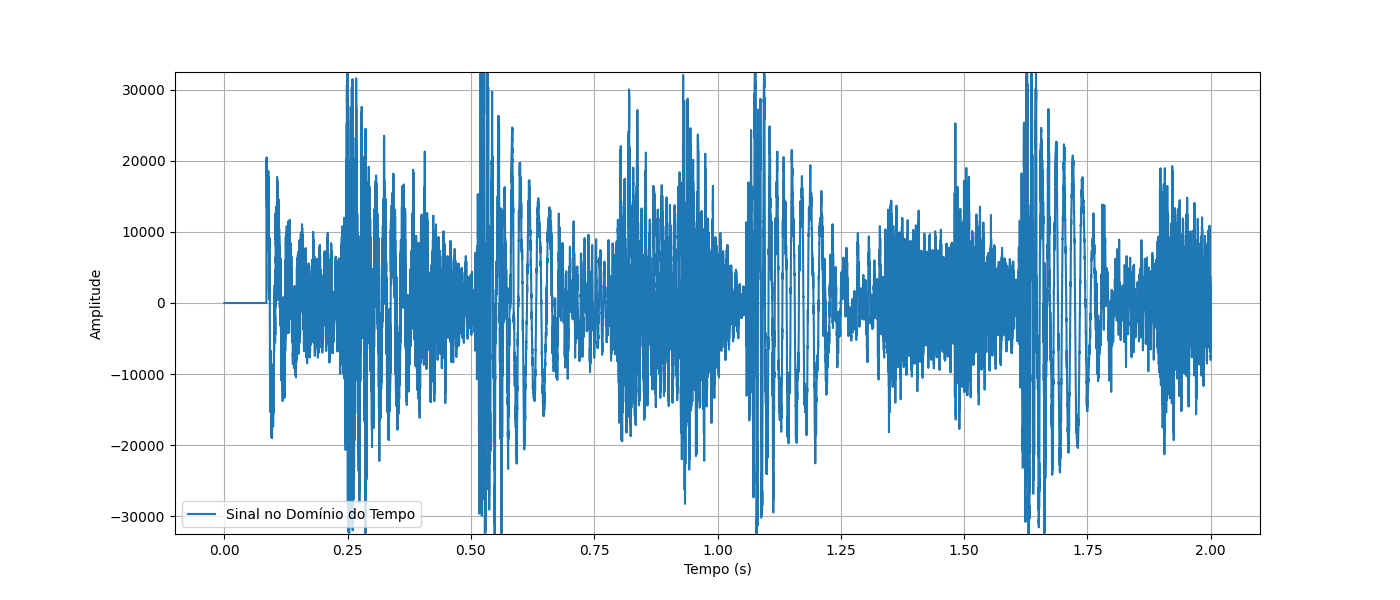
\includegraphics[width=0.5\textwidth]{figuras/fig24.png}
	\caption{música 1 no domínio do tempo com uma $f_c$ de 20 Hz}
	\label{fig24}
\end{figure}

\begin{figure}[h]
	\centering
    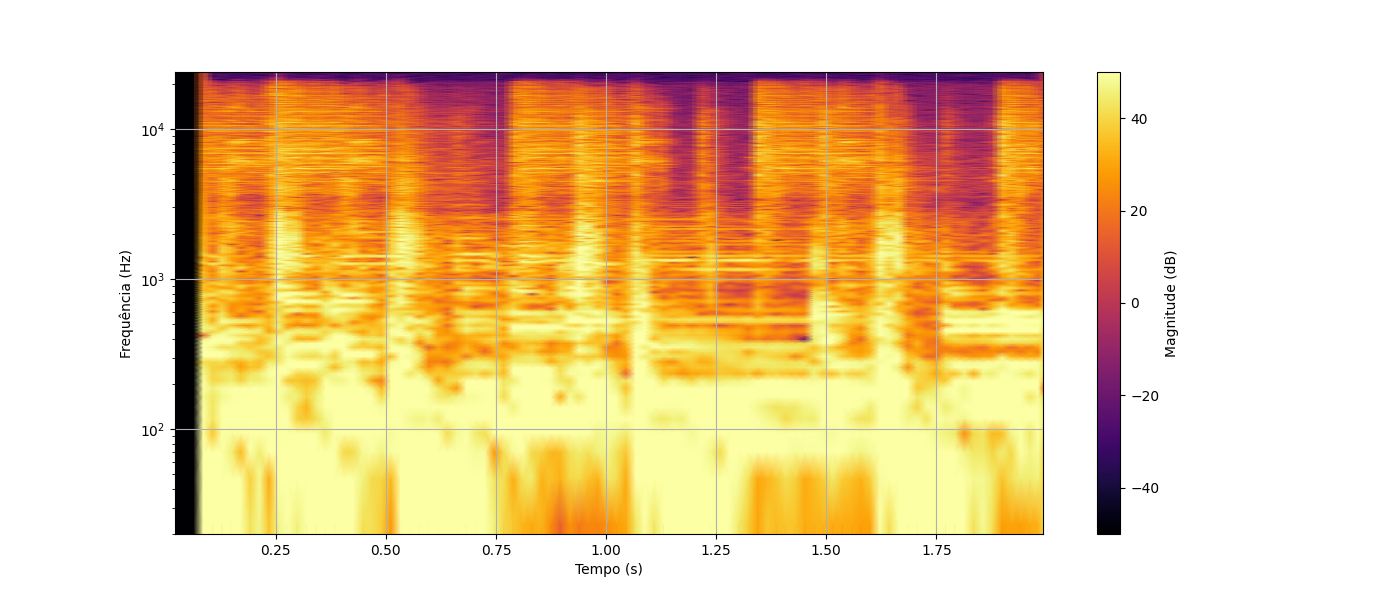
\includegraphics[width=0.5\textwidth]{figuras/fig25.png}
	\caption{música 1 no domínio da frequência com uma $f_c$ de 20 Hz}
	\label{fig25}
\end{figure}

Em mixers convencionais, o controle de ganho para baixas frequências é ajustado na banda de 300 Hz. Portanto, o controle de frequência foi ajustado para aproximar-se de 300 Hz. O resultado da filtragem está mostrado nas Figuras \ref{fig28} e \ref{fig29}.

\begin{figure}[h]
	\centering
    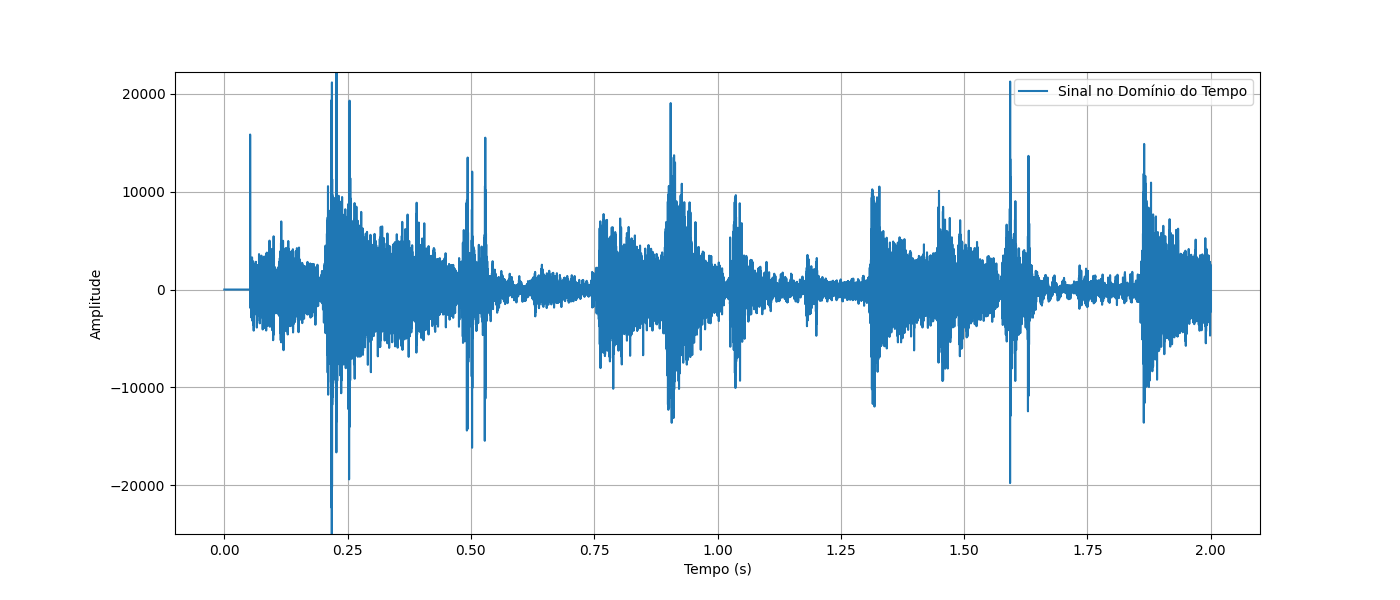
\includegraphics[width=0.5\textwidth]{figuras/fig28.png}
	\caption{música 1 no domínio do tempo com uma $f_c$ de 300 Hz}
	\label{fig28}
\end{figure}

A Figura \ref{fig28} mostra a atenuação significativa dos sinais, com a ausência de sinais de baixa frequência observados anteriormente. A Figura \ref{fig29} confirma a atenuação de sinais de baixa frequência, com uma redução aproximada de 30 dB.

\begin{figure}[h]
	\centering
    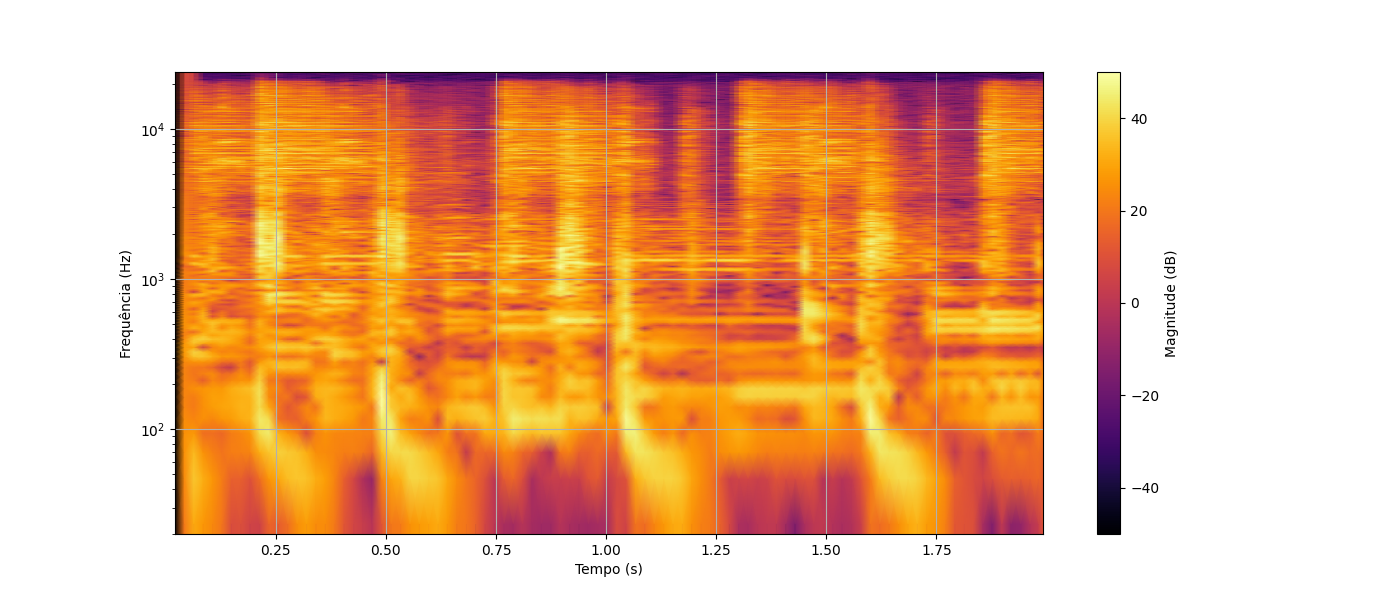
\includegraphics[width=0.5\textwidth]{figuras/fig29.png}
	\caption{música 1 no domínio da frequência com uma $f_c$ de 300 Hz}
	\label{fig29}
\end{figure}

A frequência de corte de 4 kHz, onde se encontram os elementos médios, foi aplicada em seguida. A Figura \ref{fig26} mostra a atenuação dos sinais em relação às filtragens anteriores.

\begin{figure}[h]
	\centering
    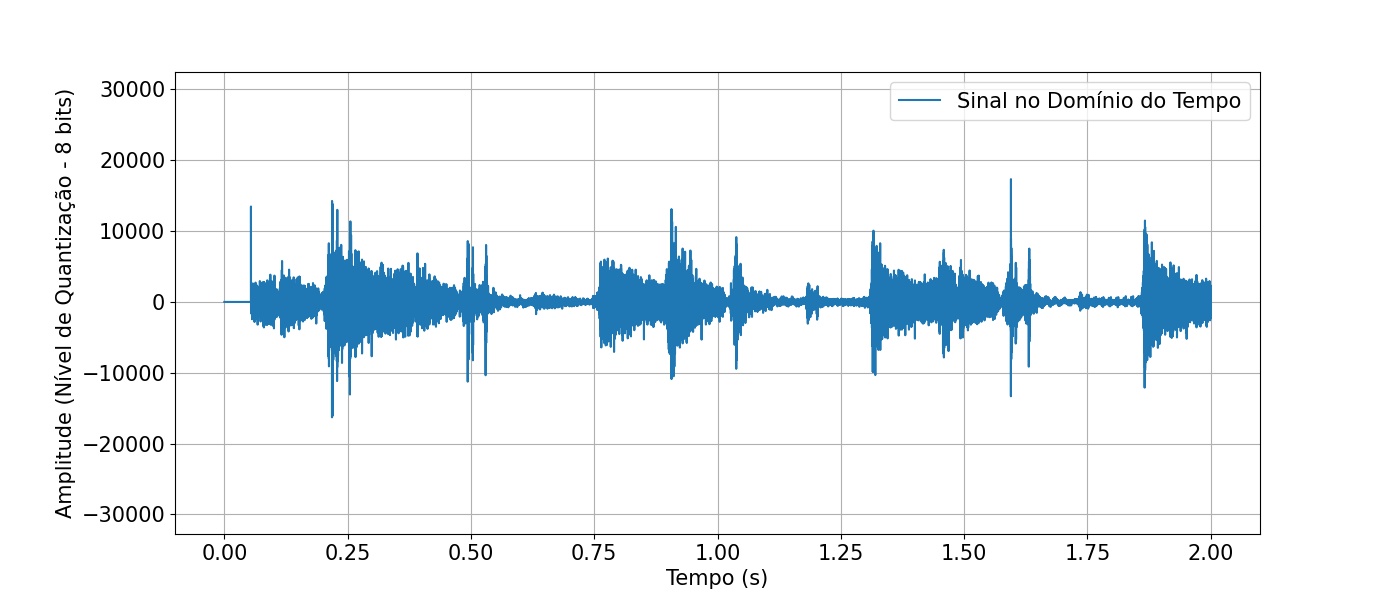
\includegraphics[width=0.5\textwidth]{figuras/fig26.png}
	\caption{música 1 no domínio do tempo com uma $f_c$ de 4 kHz}
	\label{fig26}
\end{figure}

Na Figura \ref{fig27}, a STFT revela a atenuação das componentes referentes à banda de frequência de 4 kHz, com algumas componentes atingindo 0 dB.

\begin{figure}[h]
	\centering
    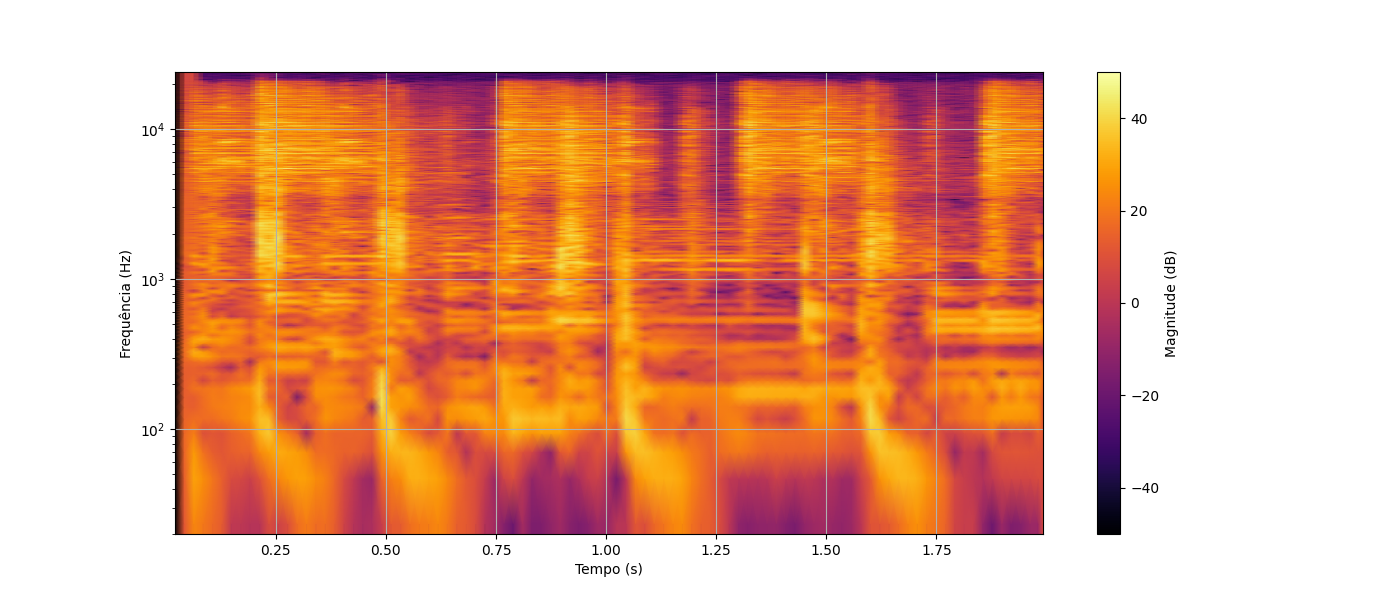
\includegraphics[width=0.5\textwidth]{figuras/fig27.png}
	\caption{música 1 no domínio da frequência com uma $f_c$ de 4 kHz}
	\label{fig27}
\end{figure}

Uma frequência de corte de 24 kHz foi utilizada para a filtragem completa da banda. A Figura \ref{fig30} mostra a atenuação das amplitudes de sinais em comparação com as filtragens anteriores.

\begin{figure}[h]
	\centering
    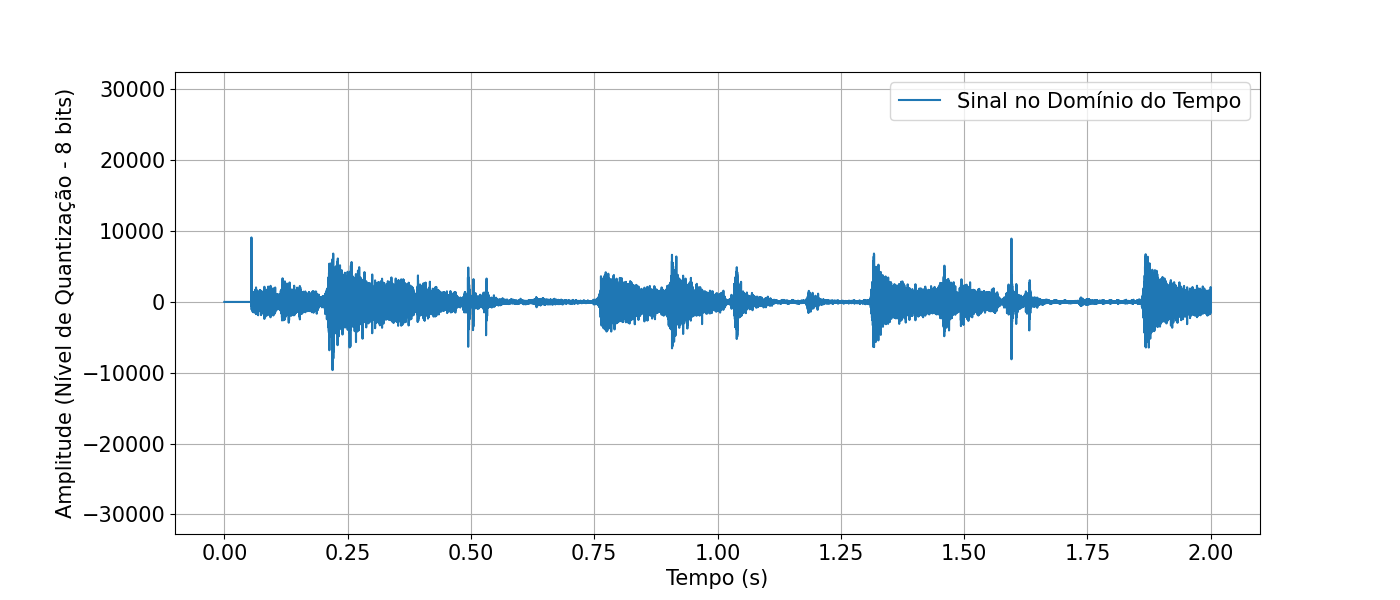
\includegraphics[width=0.5\textwidth]{figuras/fig30.png}
	\caption{música 1 no domínio do tempo com uma $f_c$ de 24 kHz}
	\label{fig30}
\end{figure}

A Figura \ref{fig31} demonstra a atenuação da banda correspondente, com elementos variando de 10 dB a -40 dB. Comparada com a STFT da filtragem anterior, observa-se uma atenuação generalizada do sinal.

\begin{figure}[h]
	\centering
    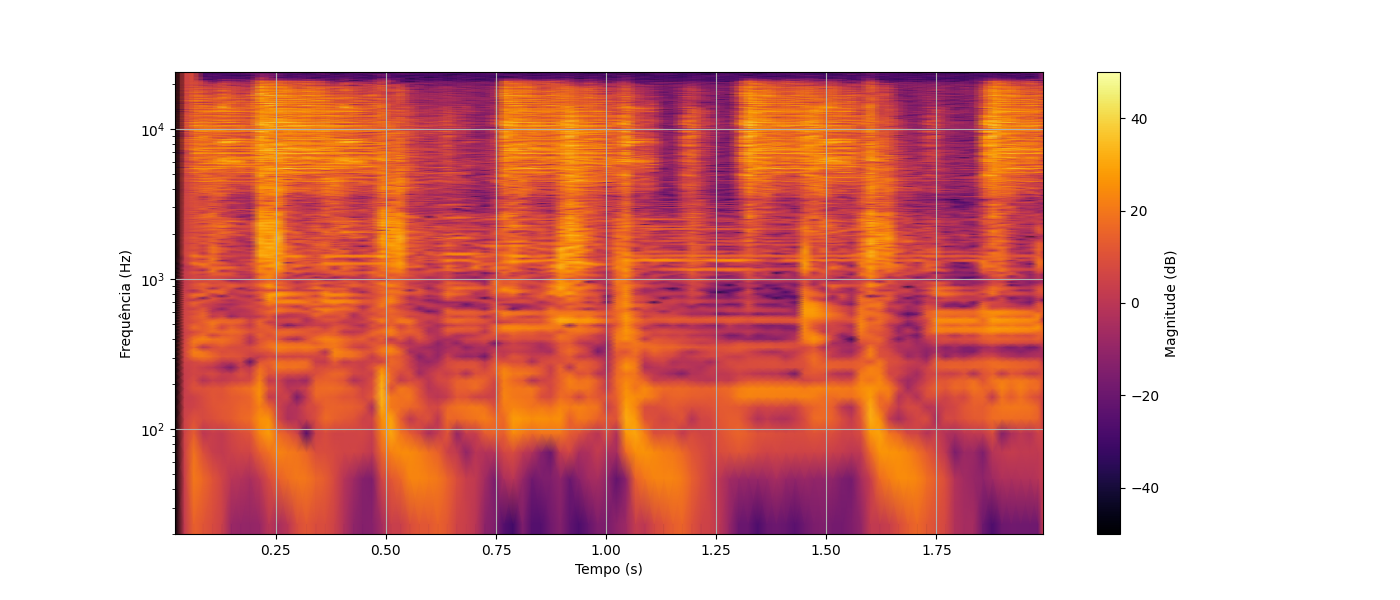
\includegraphics[width=0.5\textwidth]{figuras/fig31.png}
	\caption{música 1 no domínio da frequência com uma $f_c$ de 24 kHz}
	\label{fig31}
\end{figure}

A mesma análise foi realizada para a Música \cite{track02}. Os resultados no domínio do tempo e da frequência, utilizando a STFT, mostraram comportamentos semelhantes ao esperado.
aaaaaaaaaaaaaaaaaa
pqp meu cu
aaaaaaaaaaaaaaaaaaa
aaaaaaaaaaaaaaaaaaa
aaaaaaaaaaaaaaaaaaa
aaaaaaaaaaaaaaaaaaa
aaaaaaaaaaaaaaaaaaa

aaaaaaaaaaaaaaaaaa
\newpage
\newpage
\section{Resultados de Efeitos}

\subsection{Automação de Efeitos}

1) Inserir gráficos de presença de efeitos conforme a $f_c$ dos mixers.

2) O plot deve ser obtido variando a $f_c$ e obtendo o sinal isolado advindo dos efeitos.

3) Escolher intervalos discretos para $f_c$ conforme a proposta [fc1, fc2, fc3, fc4].

4) Comparar a presença dos efeitos em relação ao plot de presença.

\subsection{\textit{Reverb}}

Aqui, escolher-se-á a maior $f_c$ para gerar a maior presença de efeitos. Selecionar um intervalo discreto de presença de efeitos que permita visualizar a mudança de efeitos.

No caso do reverb, a quantidade de dB existente da música depois de 1 ms é utilizada, variando de 0 a 100 dB. Escolher valores de parâmetro e obter o sinal de saída isolado do efeito.

\subsection{\textit{Delay}}

No caso do delay, utilizar o mesmo conjunto de valores de parâmetros. O parâmetro a ser modificado é o tempo em ms, cuja cópia do sinal estará presente.

Substitua 0.5 por 0.1 conforme necessário.
